The fast multipole method was developed by Leslie \textsc{Greengard} and Vladimir \textsc{Rohlin} in their seminal paper \emph{A Fast Algorithm for Particle Simulations}.%
\footnote{%
        \cite{greengard1987fast} \textsc{Greengard} \& \textsc{Rohlin} (1987)
}
The application was manyparticle systems, interstellar mechanics and electrostatics being the immediate examples thereof.
Consider a swath of electrically charged particles gathered in clusters at some locations, and spread war apart in others.
By the law of \textsc{Coloumb} governing the physics of charged particle interaction, the force impressed upon some particle by all the others depends on its distance thereto.
The idea of the fast multipole method is to systematically evaluate the influence of faraway sources on a point by aggregating their influence, and calculating them in bulk.
This is done through space octree partitioning.
Whatever influence an aggregate of points children nodes have are passed onto the parent, and the influence of the parent is calculated instead.
This is efficient computationally because a lot of the required calculation for each panel is already done.
\begin{figure}[h]
  \centering
  \begin{subfigure}{.49\textwidth}
    \centering
    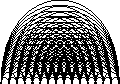
\includegraphics[scale = 3]{bem_influence.pdf}
    \caption{Direct interactions.}
  \end{subfigure}
  \begin{subfigure}{.49\textwidth}
    \centering
    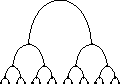
\includegraphics[scale = 3]{fmm_influence.pdf}
    \caption{Tree-based interactions.}
  \end{subfigure}
  \caption{
        The difference in number of interactions for the direct and tree-based approaches.%
        \footnote{%
                \cite{liu2009fast} \textsc{Liu}, fig.3.1, p.49, adapted with permission from author.
        }
  }
\end{figure}
